\documentclass{standalone}
\usepackage{tikz}
\usepackage{amsmath}
\usepackage{amssymb}
\long\def\gray#1{\bgroup \color{gray}#1\egroup}
\usetikzlibrary{matrix,positioning}
\usetikzlibrary{decorations.pathreplacing}

\begin{document}

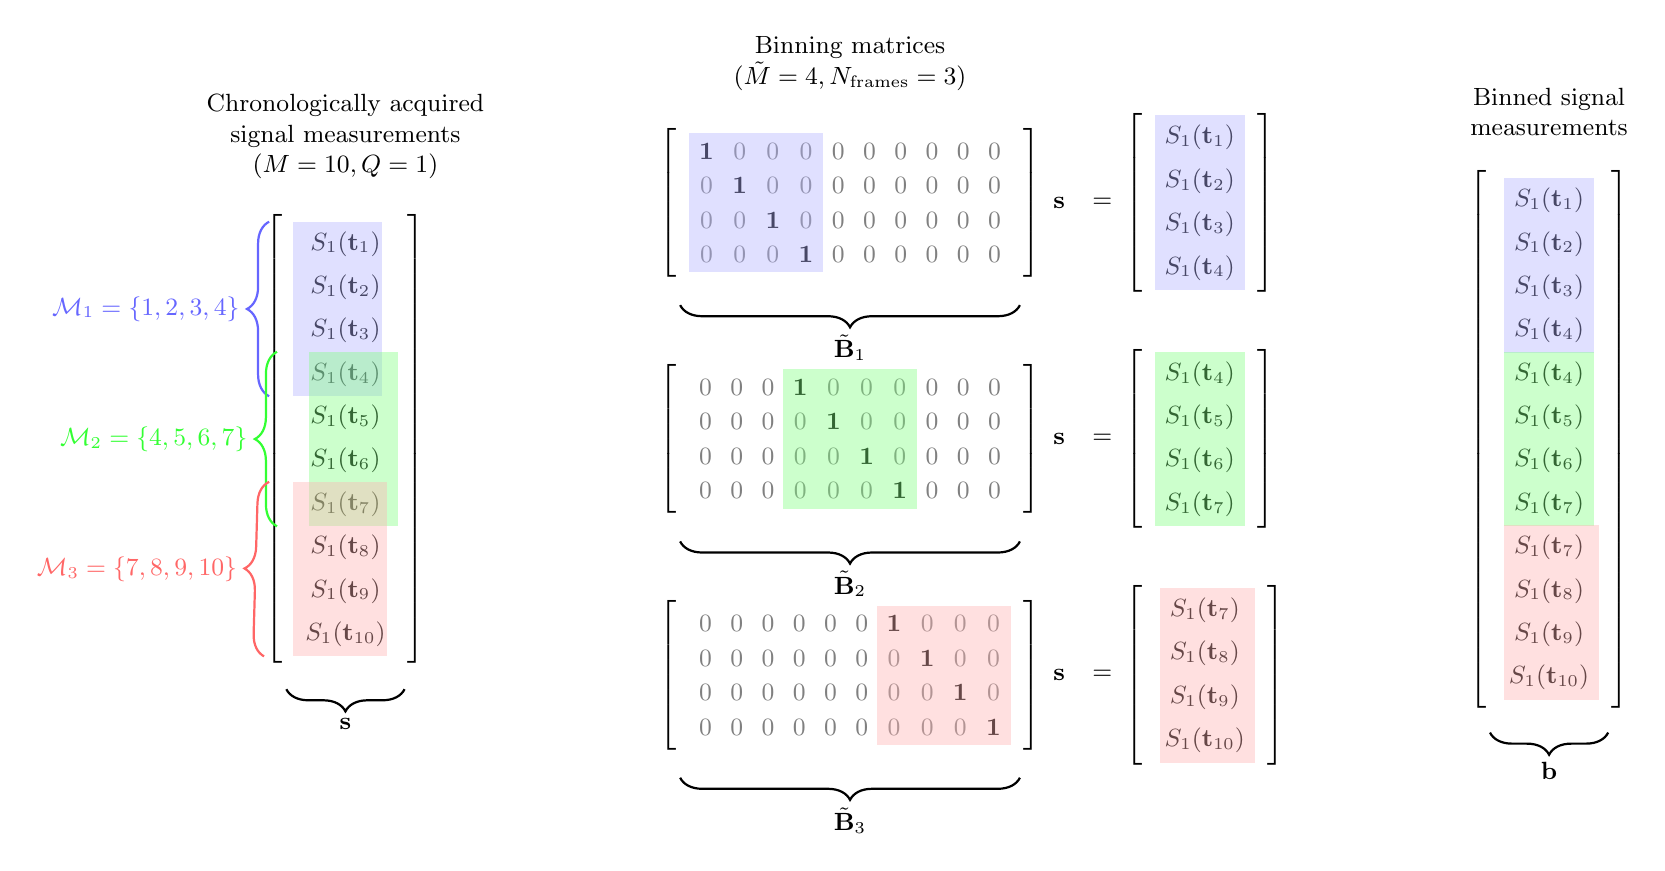
\begin{tikzpicture}[every node/.style={font=\small},node distance=2.5cm]

% Raw signal vector s
\matrix (svec) [matrix of math nodes,left delimiter={[},right delimiter={]},nodes in empty cells] {
    S_1(\mathbf{t}_1) \\
    S_1(\mathbf{t}_2) \\
    S_1(\mathbf{t}_3) \\
    S_1(\mathbf{t}_4) \\
    S_1(\mathbf{t}_5) \\
    S_1(\mathbf{t}_6) \\
    S_1(\mathbf{t}_7) \\
    S_1(\mathbf{t}_8) \\
    S_1(\mathbf{t}_9) \\
    S_1(\mathbf{t}_{10}) \\
};
\draw [decorate,decoration={brace,mirror,amplitude=8pt},thick]([yshift=-0.3cm]svec.south west) -- ([yshift=-0.3cm]svec.south east)
  node[midway,below=7pt]{$\mathbf{s}$};
\node[above=0.3cm of svec.north,align=center]{Chronologically acquired \\ signal measurements \\ ($M=10,Q=1$)};
% Draw semi-transparent rectangle around the first 4 elements
\begin{scope}
\filldraw[fill=blue!30, opacity=0.4, draw=none]
  ([xshift=-0.1cm,yshift=0.0cm]svec-1-1.north west) rectangle
  ([xshift=-0.1cm,yshift=-0.0cm]svec-4-1.south east);
\end{scope}
\begin{scope}
\filldraw[fill=green!50, opacity=0.4, draw=none]
  ([xshift=0.1cm,yshift=0.0cm]svec-4-1.north west) rectangle
  ([xshift=0.1cm,yshift=-0.0cm]svec-7-1.south east);
\end{scope}
\begin{scope}
\filldraw[fill=red!30, opacity=0.4, draw=none]
  ([xshift=-0.1cm,yshift=0.0cm]svec-7-1.north west) rectangle
  ([xshift=-0.1cm,yshift=-0.0cm]svec-10-1.south east);
\end{scope}
\draw [decorate,decoration={brace,mirror,amplitude=8pt},thick,blue!60]
  ([xshift=-0.4cm]svec-1-1.north west) -- ([xshift=-0.4cm]svec-4-1.south west)
  node[midway,left=7pt] {$\mathcal{M}_1 = \{1,2,3,4\}$};
\draw [decorate,decoration={brace,mirror,amplitude=8pt},thick,green!80]
  ([xshift=-0.3cm]svec-4-1.north west) -- ([xshift=-0.3cm]svec-7-1.south west)
  node[midway,left=7pt] {$\mathcal{M}_2 = \{4,5,6,7\}$};
\draw [decorate,decoration={brace,mirror,amplitude=8pt},thick,red!60]
  ([xshift=-0.4cm]svec-7-1.north west) -- ([xshift=-0.4cm]svec-10-1.south west)
  node[midway,left=7pt] {$\mathcal{M}_3 = \{7,8,9,10\}$};

% Binning matrices
\matrix (B2) [matrix of math nodes,right=of svec,left delimiter={[},right delimiter={]},xshift=1cm,nodes in empty cells] {
    \gray{0} & \gray{0} & \gray{0} & \mathbf{1} & \gray{0} & \gray{0} & \gray{0} & \gray{0} & \gray{0} & \gray{0} \\
    \gray{0} & \gray{0} & \gray{0} & \gray{0} & \mathbf{1} & \gray{0} & \gray{0} & \gray{0} & \gray{0} & \gray{0} \\
    \gray{0} & \gray{0} & \gray{0} & \gray{0} & \gray{0} & \mathbf{1} & \gray{0} & \gray{0} & \gray{0} & \gray{0} \\
    \gray{0} & \gray{0} & \gray{0} & \gray{0} & \gray{0} & \gray{0} & \mathbf{1} & \gray{0} & \gray{0} & \gray{0} \\
};
\node(smult2)[right=0.3cm of B2.east]{$\mathbf{s}$};
\begin{scope}
\filldraw[fill=green!50, opacity=0.4, draw=none]
  ([xshift=0.0cm,yshift=0.0cm]B2-1-4.north west) rectangle
  ([xshift=0.0cm,yshift=0.0cm]B2-4-7.south east);
\end{scope}
\node(eq2)[right=0.1cm of smult2.east]{$=$};
\matrix (sbin2) [right=0.3cm of eq2.east,matrix of math nodes,left delimiter={[},right delimiter={]},nodes in empty cells] {
    S_1(\mathbf{t}_4) \\
    S_1(\mathbf{t}_5) \\
    S_1(\mathbf{t}_6) \\
    S_1(\mathbf{t}_7) \\
};
\begin{scope}
\filldraw[fill=green!50, opacity=0.4, draw=none]
  ([xshift=0.0cm,yshift=0cm]sbin2-1-1.north west) rectangle
  ([xshift=0.0cm,yshift=0cm]sbin2-4-1.south east);
\end{scope}

\matrix (B1) [matrix of math nodes, above=1cm of B2,left delimiter={[},right delimiter={]},xshift=0cm, nodes in empty cells] {
    \mathbf{1} & \gray{0} & \gray{0} & \gray{0} & \gray{0} & \gray{0} & \gray{0} & \gray{0} & \gray{0} & \gray{0} \\
    \gray{0} & \mathbf{1} & \gray{0} & \gray{0} & \gray{0} & \gray{0} & \gray{0} & \gray{0} & \gray{0} & \gray{0} \\
    \gray{0} & \gray{0} & \mathbf{1} & \gray{0} & \gray{0} & \gray{0} & \gray{0} & \gray{0} & \gray{0} & \gray{0} \\
    \gray{0} & \gray{0} & \gray{0} & \mathbf{1} & \gray{0} & \gray{0} & \gray{0} & \gray{0} & \gray{0} & \gray{0} \\
};
\node(smult1)[right=0.3cm of B1.east]{$\mathbf{s}$};
\begin{scope}
\filldraw[fill=blue!30, opacity=0.4, draw=none]
  ([xshift=0.0cm,yshift=0cm]B1-1-1.north west) rectangle
  ([xshift=0.0cm,yshift=0cm]B1-4-4.south east);
\end{scope}
\node(eq1)[right=0.1cm of smult1.east]{$=$};
\matrix (sbin1) [right=0.3cm of eq1.east,matrix of math nodes,left delimiter={[},right delimiter={]},nodes in empty cells] {
    S_1(\mathbf{t}_1) \\
    S_1(\mathbf{t}_2) \\
    S_1(\mathbf{t}_3) \\
    S_1(\mathbf{t}_4) \\
};
\begin{scope}
\filldraw[fill=blue!30, opacity=0.4, draw=none]
  ([xshift=0.0cm,yshift=0cm]sbin1-1-1.north west) rectangle
  ([xshift=0.0cm,yshift=0cm]sbin1-4-1.south east);
\end{scope}

\matrix (B3) [matrix of math nodes, below=1cm of B2,left delimiter={[},right delimiter={]},xshift=0cm, nodes in empty cells] {
    \gray{0} & \gray{0} & \gray{0} & \gray{0} & \gray{0} & \gray{0} & \mathbf{1} & \gray{0} & \gray{0} & \gray{0} \\
    \gray{0} & \gray{0} & \gray{0} & \gray{0} & \gray{0} & \gray{0} & \gray{0} & \mathbf{1} & \gray{0} & \gray{0} \\
    \gray{0} & \gray{0} & \gray{0} & \gray{0} & \gray{0} & \gray{0} & \gray{0} & \gray{0} & \mathbf{1} & \gray{0} \\
    \gray{0} & \gray{0} & \gray{0} & \gray{0} & \gray{0} & \gray{0} & \gray{0} & \gray{0} & \gray{0} & \mathbf{1} \\
};
\node(smult3)[right=0.3cm of B3.east]{$\mathbf{s}$};
\begin{scope}
\filldraw[fill=red!30, opacity=0.4, draw=none]
  ([xshift=0.0cm,yshift=0cm]B3-1-7.north west) rectangle
  ([xshift=0.0cm,yshift=0cm]B3-4-10.south east);
\end{scope}
\node(eq3)[right=0.1cm of smult3.east]{$=$};
\matrix (sbin3) [right=0.3cm of eq3.east,matrix of math nodes,left delimiter={[},right delimiter={]},nodes in empty cells] {
    S_1(\mathbf{t}_7) \\
    S_1(\mathbf{t}_8) \\
    S_1(\mathbf{t}_9) \\
    S_1(\mathbf{t}_{10}) \\
};
\begin{scope}
\filldraw[fill=red!30, opacity=0.4, draw=none]
  ([xshift=0.0cm,yshift=0cm]sbin3-1-1.north west) rectangle
  ([xshift=0.0cm,yshift=0cm]sbin3-4-1.south east);
\end{scope}

\node[above=0.3cm of B1.north,align=center]{Binning matrices \\ ($\tilde{M}=4, N_\mathrm{frames}=3$)};

\draw [decorate,decoration={brace,mirror,amplitude=8pt},thick]([yshift=-0.3cm]B1.south west) -- ([yshift=-0.3cm]B1.south east)
  node[midway,below=7pt]{$\tilde{\mathbf{B}}_1$};
\draw [decorate,decoration={brace,mirror,amplitude=8pt},thick]([yshift=-0.3cm]B2.south west) -- ([yshift=-0.3cm]B2.south east)
  node[midway,below=7pt]{$\tilde{\mathbf{B}}_2$};
\draw [decorate,decoration={brace,mirror,amplitude=8pt},thick]([yshift=-0.3cm]B3.south west) -- ([yshift=-0.3cm]B3.south east)
  node[midway,below=7pt]{$\tilde{\mathbf{B}}_3$};
  
% Raw signal vector s
\matrix (bvec) [right=3cm of sbin2, matrix of math nodes,left delimiter={[},right delimiter={]},nodes in empty cells] {
    S_1(\mathbf{t}_1) \\
    S_1(\mathbf{t}_2) \\
    S_1(\mathbf{t}_3) \\
    S_1(\mathbf{t}_4) \\
    S_1(\mathbf{t}_4) \\
    S_1(\mathbf{t}_5) \\
    S_1(\mathbf{t}_6) \\
    S_1(\mathbf{t}_7) \\
    S_1(\mathbf{t}_7) \\
    S_1(\mathbf{t}_8) \\
    S_1(\mathbf{t}_9) \\
    S_1(\mathbf{t}_{10}) \\
};
\draw [decorate,decoration={brace,mirror,amplitude=8pt},thick]([yshift=-0.3cm]bvec.south west) -- ([yshift=-0.3cm]bvec.south east)
  node[midway,below=7pt]{$\mathbf{b}$};
\node[above=0.3cm of bvec.north,align=center]{Binned signal \\ measurements};
% Draw semi-transparent rectangle around the first 4 elements
\begin{scope}
\filldraw[fill=blue!30, opacity=0.4, draw=none]
  ([xshift=0cm,yshift=0.0cm]bvec-1-1.north west) rectangle
  ([xshift=0cm,yshift=-0.0cm]bvec-4-1.south east);
\end{scope}
\begin{scope}
\filldraw[fill=green!50, opacity=0.4, draw=none]
  ([xshift=0cm,yshift=0.0cm]bvec-5-1.north west) rectangle
  ([xshift=0cm,yshift=-0.0cm]bvec-8-1.south east);
\end{scope}
\begin{scope}
\filldraw[fill=red!30, opacity=0.4, draw=none]
  ([xshift=0cm,yshift=0.0cm]bvec-9-1.north west) rectangle
  ([xshift=0cm,yshift=0.0cm]bvec-12-1.south east);
\end{scope}

\end{tikzpicture}

\end{document}